% Importado desde: 2026-03-28_Anisotropias_Controladas_y_Geometria_Efectiva.tex
\chapter{Anisotropias controladas y geometria efectiva: --- del subsector Dirac al protoespacio deformado}
\label{ch:anisotropias-geometria-efectiva}

\begin{abstract}
El paso siguiente despues de estudiar deformaciones suaves generales es fijar una familia concreta y controlable. La opcion mas limpia es permitir velocidades diferentes en las tres direcciones espaciales, \(v_x\neq v_y\neq v_z\), manteniendo linealidad infrarroja y estructura espinorial. Este documento muestra paso a paso que esa anisotropia no destruye automaticamente el sector Dirac: primero lo convierte en una version anisotropa que puede reinterpretarse geometricamente mediante una metrica espacial efectiva o, de forma mas prudente, mediante una triada efectiva. Esa reinterpretacion es importante porque conecta las deformaciones del protoespacio con una geometria infrarroja emergente sin identificar todavia esa geometria con la del espacio-tiempo fisico completo.
\end{abstract}

\section{Pregunta concreta}
En el capitulo anterior vimos que una deformacion suave de la regla de paso puede llevar a un Hamiltoniano efectivo del tipo
\begin{equation}
H_D^{\mathrm{eff}}
=
\tau_z\otimes\left(\sum_{i,j}v_{ij}\sigma_i p_j\right)
+ m\,\tau_x\otimes \bbI_2
+ \cdots.
\end{equation}

La familia mas simple no trivial consiste en suponer que la matriz \(v_{ij}\) ya es diagonal:
\begin{equation}
v_{ij}=
\begin{pmatrix}
v_x & 0 & 0\\
0 & v_y & 0\\
0 & 0 & v_z
\end{pmatrix}.
\end{equation}

Entonces el Hamiltoniano toma la forma
\begin{equation}
H_{\mathrm{aniso}}
=
\tau_z\otimes\left(v_x\sigma_x p_x + v_y\sigma_y p_y + v_z\sigma_z p_z\right)
+ m\,\tau_x\otimes\bbI_2.
\label{c22:eq:Haniso}
\end{equation}

La pregunta es:
\begin{quote}
\textbf{que significa geometricamente que las tres velocidades efectivas no coincidan?}
\end{quote}

\section{El modelo anisotropo paso a paso}
\subsection{Bloque de Weyl}
Empecemos por un solo bloque de Weyl:
\begin{equation}
H_W^{\mathrm{aniso}}
=
v_x\sigma_x p_x + v_y\sigma_y p_y + v_z\sigma_z p_z.
\label{c22:eq:WeylAniso}
\end{equation}

Como las matrices de Pauli siguen satisfaciendo
\begin{equation}
\{\sigma_i,\sigma_j\}=2\delta_{ij}\bbI,
\end{equation}
el cuadrado del Hamiltoniano es
\begin{equation}
\left(H_W^{\mathrm{aniso}}\right)^2
=
v_x^2 p_x^2 + v_y^2 p_y^2 + v_z^2 p_z^2.
\end{equation}

Por tanto el espectro sigue siendo lineal:
\begin{equation}
E_\pm(\vp)=\pm\sqrt{v_x^2 p_x^2 + v_y^2 p_y^2 + v_z^2 p_z^2}.
\label{c22:eq:dispersionAniso}
\end{equation}

La primera leccion es directa:
\begin{quote}
\textbf{la anisotropia no destruye el nodo; deforma la forma del cono.}
\end{quote}

\begin{figure}[h!]
\centering
\begin{tikzpicture}[scale=1.0,>=Latex]
  \draw[->] (-2.8,0) -- (2.8,0) node[below] {$p_x$};
  \draw[->] (0,-0.2) -- (0,2.8) node[left] {$E$};
  \draw[thick,blue!70] (-2.2,2.2) -- (0,0) -- (2.2,2.2);
  \node[blue!70] at (1.4,1.4) {isotropo};

  \begin{scope}[xshift=6.2cm]
    \draw[->] (-2.8,0) -- (2.8,0) node[below] {$p_x$};
    \draw[->] (0,-0.2) -- (0,2.8) node[left] {$E$};
    \draw[thick,red!75!black] (-2.5,2.2) -- (0,0) -- (2.5,2.2);
    \node[red!75!black] at (1.6,1.4) {anisotropo};
  \end{scope}
\end{tikzpicture}
\caption{En una seccion fija del espacio de momentos, la anisotropia cambia la pendiente del cono sin destruir la linealidad local.}
\end{figure}

\subsection{Bloque de Dirac}
Al ensamblar dos sectores de quiralidad opuesta con masa, obtenemos \eqref{c22:eq:Haniso}. El cuadrado vale
\begin{equation}
H_{\mathrm{aniso}}^2
=
\left(v_x^2 p_x^2 + v_y^2 p_y^2 + v_z^2 p_z^2 + m^2\right)\bbI_4,
\end{equation}
de modo que
\begin{equation}
E_\pm(\vp)=\pm\sqrt{v_x^2 p_x^2 + v_y^2 p_y^2 + v_z^2 p_z^2 + m^2}.
\label{c22:eq:DiracDispersionAniso}
\end{equation}

Esto confirma que seguimos teniendo un sector tipo Dirac, aunque ya no con simetria espacial isotropa exacta.

\section{Reescalamiento de coordenadas}
\subsection{Idea basica}
Si todos los \(v_i\) son positivos y no nulos, podemos definir nuevas variables de momento
\begin{equation}
\pi_x=v_x p_x,\qquad
\pi_y=v_y p_y,\qquad
\pi_z=v_z p_z.
\label{c22:eq:piVariables}
\end{equation}

En terminos de estas variables,
\begin{equation}
H_W^{\mathrm{aniso}}
=
\sigma_x \pi_x + \sigma_y \pi_y + \sigma_z \pi_z,
\end{equation}
y
\begin{equation}
H_{\mathrm{aniso}}
=
\tau_z\otimes(\sigma_x\pi_x+\sigma_y\pi_y+\sigma_z\pi_z)
+m\,\tau_x\otimes\bbI_2.
\end{equation}

Formalmente parece que la anisotropia desaparecio. Pero en realidad no desaparecio: fue absorbida en la relacion entre \(\vp\) y \(\bm{\pi}\).

\subsection{Significado}
Esto nos enseña algo muy importante:
\begin{quote}
\textbf{una anisotropia diagonal puede verse como un cambio de escala entre las direcciones espaciales efectivas.}
\end{quote}

Es decir, el sector espinorial no \enquote{ve} las tres direcciones con la misma rigidez dinamica. El protoespacio se manifiesta en el infrarrojo como una geometria espacial deformada.

\section{Interpretacion mediante una metrica espacial efectiva}
\subsection{Forma cuadratica}
La relacion de dispersion \eqref{c22:eq:dispersionAniso} puede escribirse como
\begin{equation}
E^2 = g_{\mathrm{eff}}^{ij} p_i p_j,
\end{equation}
con
\begin{equation}
g_{\mathrm{eff}}^{ij}
=
\begin{pmatrix}
v_x^2 & 0 & 0\\
0 & v_y^2 & 0\\
0 & 0 & v_z^2
\end{pmatrix}.
\label{c22:eq:geffcontr}
\end{equation}

En el caso con masa,
\begin{equation}
E^2 = g_{\mathrm{eff}}^{ij} p_i p_j + m^2.
\end{equation}

\subsection{Interpretacion prudente}
No debemos decir demasiado rapido que ya tenemos la metrica del espacio-tiempo fisico. Lo que si podemos decir con seguridad es:
\begin{enumerate}[label=\arabic*.]
    \item el sector infrarrojo define una forma cuadratica efectiva en el espacio de momentos;
    \item esa forma cuadratica codifica la anisotropia heredada del protoespacio;
    \item la isotropia aparece cuando \(v_x=v_y=v_z\).
\end{enumerate}

Asi, una formulacion prudente es:
\begin{quote}
\textbf{la anisotropia controlada induce una geometria cinetica efectiva.}
\end{quote}

\begin{figure}[h!]
\centering
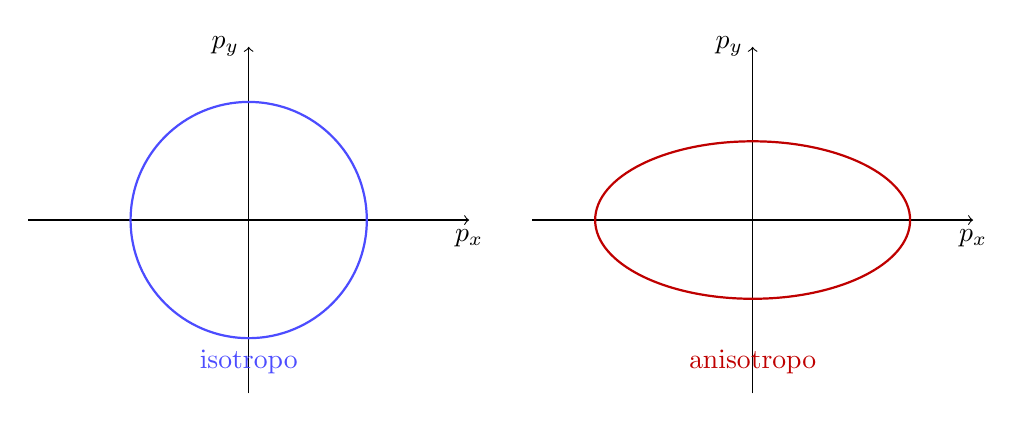
\begin{tikzpicture}[scale=1.0]
  \draw[->] (-2.8,0) -- (2.8,0) node[below] {$p_x$};
  \draw[->] (0,-2.2) -- (0,2.2) node[left] {$p_y$};
  \draw[thick,blue!70] (0,0) circle (1.5);
  \node[blue!70] at (0,-1.8) {isotropo};

  \begin{scope}[xshift=6.4cm]
    \draw[->] (-2.8,0) -- (2.8,0) node[below] {$p_x$};
    \draw[->] (0,-2.2) -- (0,2.2) node[left] {$p_y$};
    \draw[thick,red!75!black] (0,0) ellipse (2.0 and 1.0);
    \node[red!75!black] at (0,-1.8) {anisotropo};
  \end{scope}
\end{tikzpicture}
\caption{Las superficies de energia constante pasan de esferas a elipsoides en el espacio de momentos.}
\end{figure}

\section{Interpretacion mediante triadas efectivas}
Hay una lectura todavia mas cercana a la estructura espinorial. En vez de hablar primero de metrica, podemos introducir una triada efectiva \(e^a{}_i\) tal que
\begin{equation}
H_W^{\mathrm{aniso}} = \sigma_a\, e^a{}_i\, p_i.
\label{c22:eq:triadform}
\end{equation}

En nuestro caso diagonal,
\begin{equation}
e^a{}_i=
\begin{pmatrix}
v_x & 0 & 0\\
0 & v_y & 0\\
0 & 0 & v_z
\end{pmatrix}.
\label{c22:eq:triadDiag}
\end{equation}

Entonces la forma cuadratica efectiva se reconstruye como
\begin{equation}
g_{\mathrm{eff}}^{ij}=\delta^{ab} e^i{}_a e^j{}_b,
\end{equation}
o, equivalentemente, como la combinacion cuadratica inducida por la triada.

Esta lectura es conceptualmente muy atractiva porque:
\begin{enumerate}[label=\arabic*.]
    \item la triada acopla directamente el espacio interno espinorial con las direcciones espaciales;
    \item muestra como la fibra local y la geometria efectiva quedan entrelazadas;
    \item prepara mejor el paso a deformaciones que dependan lentamente de la posicion.
\end{enumerate}

\section{Que se preserva y que se pierde}
La anisotropia controlada preserva:
\begin{enumerate}[label=\arabic*.]
    \item la linealidad infrarroja;
    \item la estructura de Clifford local;
    \item la interpretacion en terminos de fermion de Dirac o Weyl efectivo.
\end{enumerate}

La anisotropia controlada rompe o deforma:
\begin{enumerate}[label=\arabic*.]
    \item la isotropia espacial exacta;
    \item la identificacion simple entre todas las direcciones locales;
    \item la forma mas simetrica del cono relativista efectivo.
\end{enumerate}

Eso es exactamente lo que buscabamos: una deformacion suficientemente suave como para no destruir el sector Dirac, pero suficientemente rica como para empezar a extraer informacion geometrica del protoespacio.

\section{Lectura para el programa de investigacion}
Este paso cambia el foco del proyecto de una manera muy sana.

Antes la pregunta era:
\begin{quote}
\enquote{que protoespacio produce Dirac?}
\end{quote}

Ahora la pregunta se vuelve:
\begin{quote}
\enquote{que familia de protoespacios produce una familia de geometrias efectivas vistas por el sector Dirac?}
\end{quote}

Esa reformulacion es mejor por dos razones:
\begin{enumerate}[label=\arabic*.]
    \item no exige que todo salga exactamente isotropo desde el comienzo;
    \item convierte las deformaciones del infrarrojo en observables conceptuales del protoespacio.
\end{enumerate}

\section{Siguiente paso natural}
Hay dos prolongaciones muy naturales desde aqui:
\begin{enumerate}[label=\arabic*.]
    \item permitir que \(v_x,v_y,v_z\) dependan lentamente de la posicion y del tiempo discretos;
    \item permitir terminos fuera de la diagonal en \(v_{ij}\), para estudiar cizallas y mezclas direccionales.
\end{enumerate}

La primera es la mas prometedora para la linea principal del proyecto, porque llevaria de una triada constante a una triada efectiva variable, y por tanto a una geometria emergente mas rica.

\section*{Conclusion}
El resultado central de este capitulo puede resumirse asi:
\begin{quote}
\textbf{la anisotropia controlada no mata el subsector Dirac; lo convierte en una sonda de la geometria efectiva del protoespacio.}
\end{quote}

En el caso diagonal, esa geometria puede describirse de manera sencilla por una forma cuadratica efectiva o, mejor aun, por una triada efectiva que conecta directamente la fibra espinorial con las direcciones del espacio discreto.
